\tikzset{every picture/.style={line width=0.75pt}} %set default line width to 0.75pt        

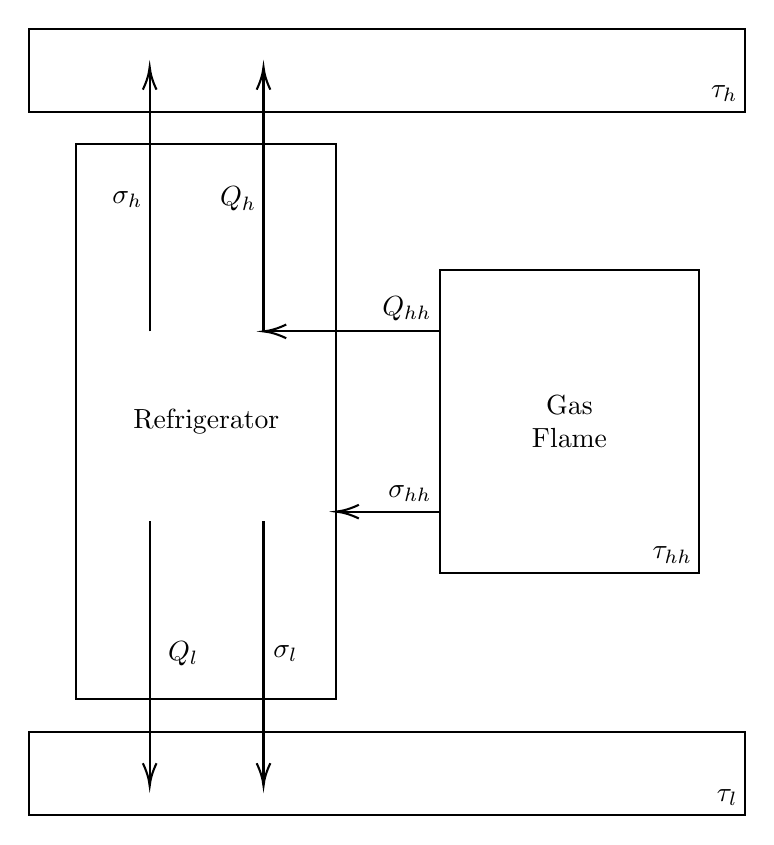
\begin{tikzpicture}[x=0.75pt,y=0.75pt,yscale=-1,xscale=1]
%uncomment if require: \path (0,444); %set diagram left start at 0, and has height of 444

%Shape: Rectangle [id:dp10170211024317433] 
\draw   (147,21) -- (492,21) -- (492,61) -- (147,61) -- cycle ;
%Shape: Rectangle [id:dp4544811596066871] 
\draw   (147,360) -- (492,360) -- (492,400) -- (147,400) -- cycle ;
%Shape: Rectangle [id:dp3842791172068818] 
\draw   (295.08,76.5) -- (295.08,344) -- (170,344) -- (170,76.5) -- cycle ;
%Shape: Rectangle [id:dp8874129257814114] 
\draw   (470.08,137.13) -- (470.08,283.38) -- (345,283.38) -- (345,137.13) -- cycle ;
%Straight Lines [id:da32858104289441736] 
\draw    (344.54,253.67) -- (297.12,253.67) ;
\draw [shift={(295.12,253.67)}, rotate = 360] [color={rgb, 255:red, 0; green, 0; blue, 0 }  ][line width=0.75]    (10.93,-3.29) .. controls (6.95,-1.4) and (3.31,-0.3) .. (0,0) .. controls (3.31,0.3) and (6.95,1.4) .. (10.93,3.29)   ;
%Straight Lines [id:da3165588536319903] 
\draw    (344.54,166.83) -- (262.12,166.83) ;
\draw [shift={(260.12,166.83)}, rotate = 360] [color={rgb, 255:red, 0; green, 0; blue, 0 }  ][line width=0.75]    (10.93,-3.29) .. controls (6.95,-1.4) and (3.31,-0.3) .. (0,0) .. controls (3.31,0.3) and (6.95,1.4) .. (10.93,3.29)   ;
%Straight Lines [id:da25070487209015857] 
\draw    (260.12,166.83) -- (260.12,41.41) ;
\draw [shift={(260.12,39.41)}, rotate = 90] [color={rgb, 255:red, 0; green, 0; blue, 0 }  ][line width=0.75]    (10.93,-3.29) .. controls (6.95,-1.4) and (3.31,-0.3) .. (0,0) .. controls (3.31,0.3) and (6.95,1.4) .. (10.93,3.29)   ;
%Straight Lines [id:da9292611993021886] 
\draw    (205.28,166.83) -- (205.28,41.41) ;
\draw [shift={(205.28,39.41)}, rotate = 90] [color={rgb, 255:red, 0; green, 0; blue, 0 }  ][line width=0.75]    (10.93,-3.29) .. controls (6.95,-1.4) and (3.31,-0.3) .. (0,0) .. controls (3.31,0.3) and (6.95,1.4) .. (10.93,3.29)   ;
%Straight Lines [id:da32161089218702354] 
\draw    (205.28,258.41) -- (205.28,383.83) ;
\draw [shift={(205.28,385.83)}, rotate = 270] [color={rgb, 255:red, 0; green, 0; blue, 0 }  ][line width=0.75]    (10.93,-3.29) .. controls (6.95,-1.4) and (3.31,-0.3) .. (0,0) .. controls (3.31,0.3) and (6.95,1.4) .. (10.93,3.29)   ;
%Straight Lines [id:da06444914845130922] 
\draw    (260.12,258.41) -- (260.12,383.83) ;
\draw [shift={(260.12,385.83)}, rotate = 270] [color={rgb, 255:red, 0; green, 0; blue, 0 }  ][line width=0.75]    (10.93,-3.29) .. controls (6.95,-1.4) and (3.31,-0.3) .. (0,0) .. controls (3.31,0.3) and (6.95,1.4) .. (10.93,3.29)   ;

% Text Node
\draw (490,57.6) node [anchor=south east] [inner sep=0.75pt]    {$\tau _{h}$};
% Text Node
\draw (490,396.6) node [anchor=south east] [inner sep=0.75pt]    {$\tau _{l}$};
% Text Node
\draw (468.08,279.97) node [anchor=south east] [inner sep=0.75pt]    {$\tau _{hh}$};
% Text Node
\draw (342.54,250.27) node [anchor=south east] [inner sep=0.75pt]    {$\sigma _{hh}$};
% Text Node
\draw (342.54,163.43) node [anchor=south east] [inner sep=0.75pt]    {$Q_{hh}$};
% Text Node
\draw (407.54,210.25) node   [align=left] {\begin{minipage}[lt]{31.07pt}\setlength\topsep{0pt}
\begin{center}
Gas \\Flame
\end{center}

\end{minipage}};
% Text Node
\draw (258.12,103.12) node [anchor=east] [inner sep=0.75pt]    {$Q_{h}$};
% Text Node
\draw (203.28,103.12) node [anchor=east] [inner sep=0.75pt]    {$\sigma _{h}$};
% Text Node
\draw (230.28,322.12) node [anchor=east] [inner sep=0.75pt]    {$Q_{l}$};
% Text Node
\draw (278.12,322.12) node [anchor=east] [inner sep=0.75pt]    {$\sigma _{l}$};
% Text Node
\draw (232.54,210.25) node   [align=left] {Refrigerator};


\end{tikzpicture}
